\section{Lithium teknologi}
Lithium batterier har siden 1973 været under konstant udvikling. Gennem tiden er der opdaget mange forskellige typer for lithium batterier. Målet er, som ved så mange andre typer batterier, at få den højeste kapacitet på mindst mulig plads. Men da der ved lithium batterier er farlige konsekvenser ved dette, er man nødt til at finde det bedste kompromis. "Hovednavnet" \space /det mest brugte navn for de mange forskellige typer er bare "lithium-ion" \space men hvis man går lidt dybere ned i kemien ser man at der findes lithium-ion batterier med mange forskellige karakteristika. 

\subsection{Forskel på kemierne}
Den nok mest brugte er dog lithium cobalt oxid-typen ($LiCoO_2$, også kaldt $LCO$) som bruges i f.eks. mobiltelefoner og moderne bærbare computere. Denne type er den mest fleksible i dens fysiske design, men også den farligste. Derfor er det vigtigt at denne type celle har et overvågningskredsløb, da der ellers kan forekomme katastrofale situationer. Disse celler er oftest formet som "bløde puder" \space \textemdash \space altså uden en hård kasse rundt om. Denne teknologi bruges også oftest i lithium ion polymer-varianten, som bliver brugt meget i RC-industrien pga. den høje afladekapacitet og den kompakte form.

\begin{figure}[h]
	\centering
	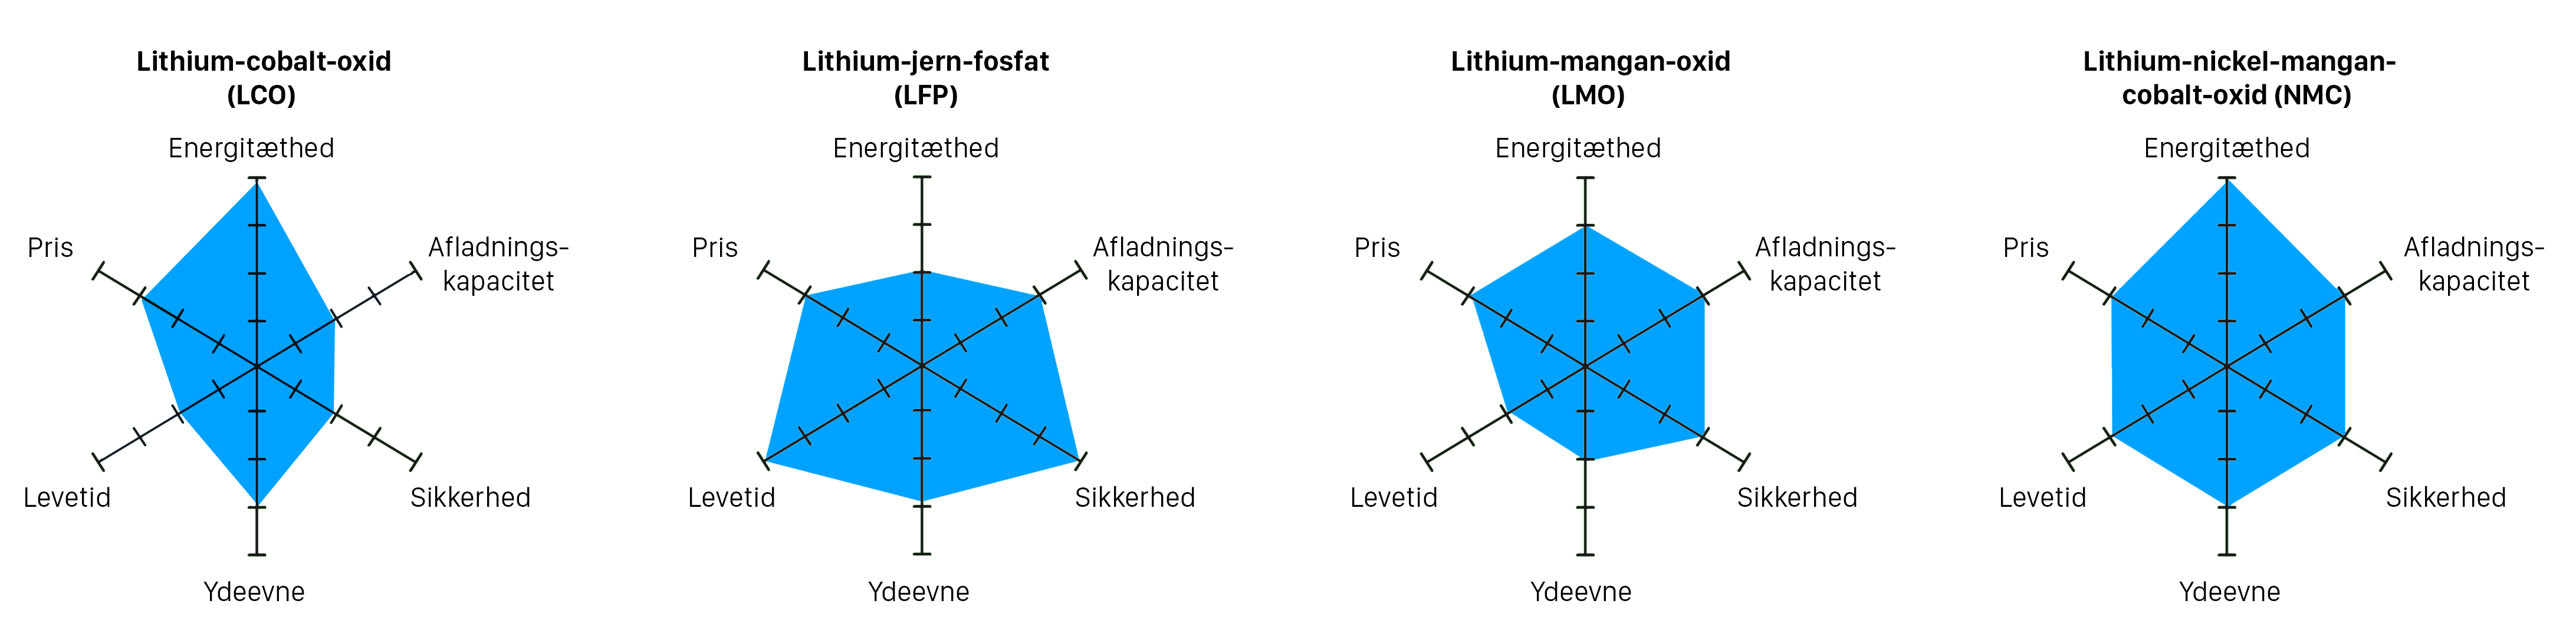
\includegraphics[width=15cm]{billeder/chemical-comparison.png}
	\caption{Sammenligning af de forskellige former for lithium ion celler\protect\footnotemark}
	\label{fig:lithium_variants_comparison}
\end{figure}
\footnotetext{BCG Research forskning i de bedste batterier til el-biler. \url{https://www.bcg.com/documents/file36615.pdf}}

\sbf{Skal måske rettes til større tekst}

Som der ses på figur \ref{fig:lithium_variants_comparison} sammenlignes de forskellige typer litium-ion kemier. Her sammenlignes energitæthed, altså hvor meget "køretid" \space cellen har; afladningskapacitet som beskriver hvor meget batteriet kan aflade med i øjeblikket; sikkerhed; ydeevne i både kolde og varme omgivelsestemperaturer; celletypens levetid/antal ladecyklusser; og pris. \\

Lithium jern fosfat ($LiFePO_4$ også kaldt $LFP$) har sammen med lithium mangan oxid ($LiMn_2O_4$ også kaldt $LMO$) og lithium nikkel mangan cobalt oxid ($LiNiMnCoO_2$ også kaldt $NMC$) en lavere energidensitet men er mere sikker end lithium cobalt oxid. De har også en længere levetid og derfor er de meget brugte i f.eks. elektrisk værktøj eller medicinindustrien. Sidstnævnte ($NMC$) er især dominerende i elektriske biler. Disse celler findes oftest i 18650 varianten, som er en rund cylindrisk celle. Det er også denne type celle der er valgt til dette projekt, da det efterhånden er en ret standard celle, og da dens karakteristika er ganske veldokumenteret. 

\begin{center}
	\setlength{\tabcolsep}{5pt}
	\begin{tabular}{| p{2.3cm} | p{2.71cm} | p{2.71cm} | p{2.71cm} | p{2.71cm} |}
		\hline
		  & $LiCoO_2$ & $LiFePO_4$ & $LiMn_2O_4$ & $LiNiMnCoO_2$ \\ \hline
		Spændinger & $3.6\volt$ nominal, typisk $3.0-4.2\volt$  & $3.2-3.3\volt$ nominal, typisk $2.5-3.65\volt$ & $3.7-3.8\volt$ nominal, typisk $3.0-4.2\volt$ & $3.6-3.7\volt$ nominal, typisk $3.0-4.2\volt$ \\ \hline
		Energitæthed & $150-250\watt\hour/\kilogram$ & $90-120\watt\hour/\kilogram$ & $100-150\watt\hour/\kilogram$ & $150-220\watt\hour/\kilogram$ \\ \hline
		Opladning & $0.7-1C$ op til $4.2\volt$ & $1C$ op til $3.65\volt$ & $0.7-1C$ (fast \space \space charge ved $3C$) op til $4.2\volt$ & $0.7-1C$ op til $4.2\volt$ \\ \hline		
		Afladning & $1C$, cut-off ved $2.5\volt$ & $1C$, nogle $25C$, cut-off ved $2.5\volt$ & $1C$, nogle $10C$, cut-off ved $2.5\volt$ & $1C$, nogle $2C$, cut-off ved $2.5\volt$ \\ \hline
		Levetid & 500-1000 cycles & 1000-2000 cycles & 300-700 cycles & 1000-2000 cycles \\ \hline
		Kritisk temperatur & $150\degreeCelsius$ & $270\degreeCelsius$ & $250\degreeCelsius$ & $210\degreeCelsius$ \\ \hline
	\end{tabular}
\end{center}

\sbf{Skriv hvilken kemi vi har valgt}

\section{Anvendelse}
Den valgte type lithium-ion celle har en nominal spænding på $3.6\volt$. "Sikkerhedszonen" \space anses for at ligge mellem $3\volt$ og $4.2\volt$. Lades cellen til mere end $4.2\volt$ tager cellen skade og mister kapacitet. Det er også over dette niveau at de katastrofale situationer kan finde sted. Det samme gælder for afladningen. Aflades cellen under $3\volt$ går det også ud over kapaciteten men ikke i samme rate. Nogle typer kan også holde til afladning ned til $2.5\volt$, så denne grænse er en smule mere udefineret.\\
\sbf{Redefiner lidt af formuleringen her}

Kigges der på en typisk 18650 celle såsom Samsung 30Q modellen, har den en afladningskurve (ved $5\ampere$) der ser ud som følgende: 

\begin{figure}[h]
\centering
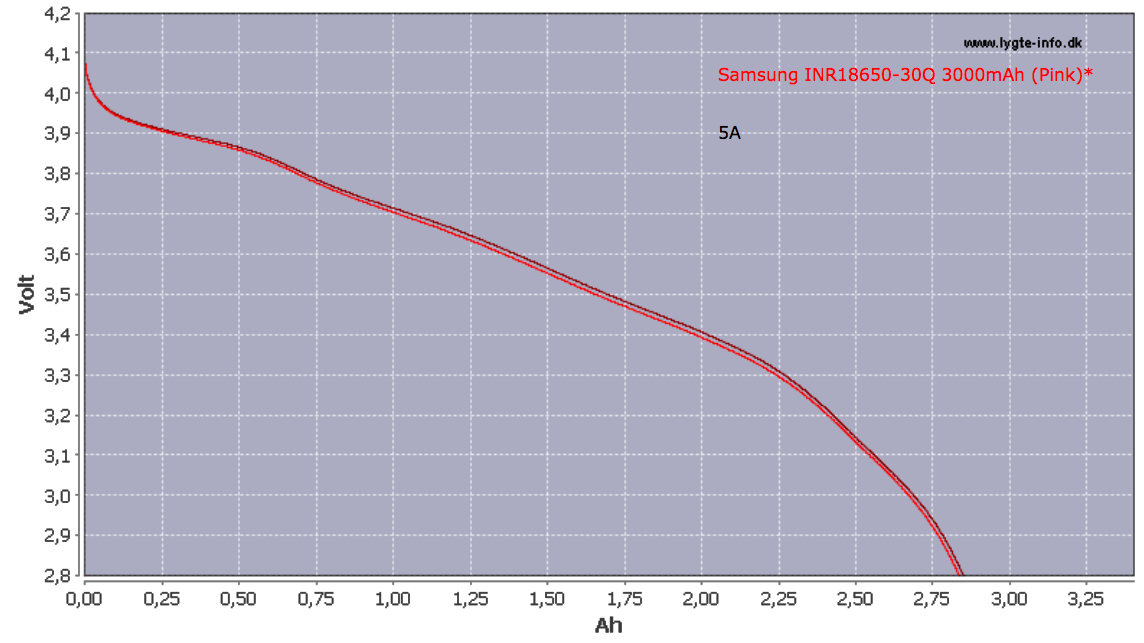
\includegraphics[width=15cm]{billeder/samsung-inr18650-discharge.png}
\caption{Afladekurven for en Samsung INR18650 30Q celle\protect\footnotemark}
\label{fig:30q_discharge}
\end{figure}
\footnotetext{Kurve fra celle-sammenligningsværktøj på Lygte Info's hjemmeside. \url{https://lygte-info.dk/review/batteries2012/Common18650comparator.php}}

Denne celle står oplyst til at have $3000\milli\ampere\hour$ men som der ses på kurven, er cellens spænding allerede på $2.8\volt$ når der er omkring $150\milli\ampere\hour$ tilbage. Derfor, hvis man holder sig inden for "sikkerhedszonen" \space udnytter man ikke batteriets fulde kapacitet, men derimod opnår man en længere levetid på cellen. \\

Skal cellerne opbevares i længere tid, er det en god idé at opbevare dem i den såkaldte "storage mode". Her lades/aflades cellerne til $30-40\percent$ af deres fulde kapacitet, da der her er mindst slid, og man derfor opnår en længere levetid. 

\sbf{Sammenlign reel kurve og lineær kurve}

\section{Sikkerhed}
Da lithium batterier kan være farlige, er man nødt til at foretage de nødvendige sikkerhedsforanstaltninger. Derfor er der en del "regler":
\begin{itemize}
\item Oplad ikke på batteriet når omgivelsestemperaturen er under $0\degreeCelsius$
\item Batteriet må ikke oplades til mere end $4.2\volt$ ($4.X\volt$ når det er $LiFePO_4$)
\item Brug helst en balance oplader eller et batteristyresystem hvis der er flere celler i serie
\item Flere punkter her
\end{itemize}
\sbf{Husk at rette lifepo4 max voltage}

Lidt om kortslutningsbeskyttelse, overophedning under opladning og afladning, måske state of health.

\section{Elektrisk model af en celle}
For at kunne udvikle et batteristyresystem er det nødvendigt, at have en model for en celle i form at et elektrisk ækvivalensdiagram. Alt afhængig af modellens kompleksitet vil databehandling af State of Charge og State of Health blive mere præcis.
\\

Den mest simple model kan tilnærme sig op- og afladningskarakteristikken for en superkondensator, hvor kurven er lineær gennem hele arbejdsområdet.

\sbf{Kom ind under den simple model og hvorfor vi har valgt den. Kenneth skriver kort om den avancerede model og dens formel, men ikke mere end det.}





